\documentclass[onecolumn,superscriptaddress,10pt,showpacs,showkeys,pla]{revtex4}%
\renewcommand\baselinestretch{2}
\usepackage{mathrsfs}%
\usepackage{natbib}
\usepackage{bm}
\usepackage{amsmath}
\usepackage{threeparttable}
\usepackage{amssymb}
\usepackage{amsfonts}
\usepackage[colorlinks,CJKbookmarks,linkcolor=blue]{hyperref}
\usepackage{color}
\usepackage{booktabs}  %���岻ͬ��ϸ�ķָ���
\usepackage{tabularx}  %������
\usepackage{graphicx}%

\begin{document}
\title{Experimentally simulating the violation of Bell-type inequalities for generalized GHZ states}

\begin{abstract}
Using NMR techniques, we simulate the violations of two Bell-type
inequalities: Mermin-Ardehali-Belinskii-Klyshko (MABK) inequality
and Chen's inequality\cite{MABK,Chen}, for the 3-qubit generalized
GHZ states. The experimental results are in good agreement with the
quantum predictions and show that Chen's inequality is more
efficient than MABK inequality in the case of the generalized GHZ
entangled states.
\end{abstract}

\maketitle

\subsection*{I. Introduction}

 In 1964, Bell showed that in all local realistic
theories, correlations between the outcomes of measurements in
different parts of a physical system satisfy a certain class of
inequalities \cite{Bell}. However, it is easy to find that entangled
states violate these inequalities in quantum mechanics, which shows
the crucial conflict between classical theory and quantum mechanics.
Hence, Bell's work was described as "the most profound discovery of
science" \cite{Stapp} or "one of the greatest discoveries of modern
science" \cite{Zukowski}. Later, more important generalizations,
including the Clauser-Horne-Shimony-Holt (CHSH) \cite{CHSH} and
Mermin-Ardehali-Belinskii-Klyshko (MABK) inequalities \cite{MABK}
were developed. Recently, Werner, Wolf, \.{Z}ukowski and Brukner
(WWZB) derived a set of multipartite Bell inequalities, using two
dichotomic observables per site \cite{WWZB}. The investigation of
Bell's inequalities exhibit fundamental problems of quantum
mechanics and also relate to quantum communication \cite{ Brukner,
Brassard, Scarani} and cryptography \cite{Chen,Acin and Gisin}, such
as the loophole-free violation of the inequalities is the basis of
the security some quantum communication protocols \cite{Acin and
Gisin,
 Acin and Brunner}. the inequalities themselves are also useful tools to detect entanglement
which is a powerful computational resource in quantum computation
\cite{Nielsen}. Obviously, further work is worth doing in this
domain. Various experiments to test Bell inequality have been
performed in various systems including photons \cite{Freedman,
Aspect, Weihs}, atoms systems \cite{Moehring}, atomic ensembles
\cite{Matsukevich3, Chou}, and trapped ions \cite{Rowe}. Recently,
an experiment to simulate the violation of CHSH inequality was
carried out on NMR \cite{Souza}. All the experiments before were
mainly implemented on the maximal entangled states, such as Bell
state and the standard GHZ state, but rarely on nonmaximal entangled
states, such as the generalized GHZ states. However, many phenomena
can only be disclosed by nonmaximal entangled states, for instance,
the nonmaximal entangled states make the maximal violation of many
Bell-type inequalities \cite{Acin and Durt, Methot and Scarani}.
There are still many open problems about the Bell-type inequalities
with nonmaximal entangled states. Therefore, it is interesting and
meaningful to study the case of nonmaximal entangled states.

For the three-qubit generalized GHZ states
\begin{equation}\label{generalized GHZ state} \left\vert
\Psi \right\rangle=\cos\theta\left\vert 000 \right\rangle+\sin
\theta\left\vert 111 \right\rangle,
\end{equation}
which $\theta\in(0, \frac{\pi}{2})$,
 Scarani and Gisin
\cite{Scarani and Gisin} firstly found that there existed a region
of them satisfying the MABK inequality. It was shown that for
$\theta\leq \pi/12$ or $\theta\geq5\pi/12$ the states
\eqref{generalized GHZ state} do not violate the three-qubit MABK
inequality. Later on, \.{Z}ukowski \emph{et.al} proved that
\cite{Zukowski and Brukner and Laskowski and Wiesniak} ($i$) for
$N=even$, the generalized GHZ states violate the WWZB inequality,
rather than MABK inequalities; ($ii$) for $N=odd$ and
$sin(2\theta)\leq1/\sqrt{2^{N-1}}$, the generalized GHZ states
satisfy both MABK and WWZB inequalities. Soon, Chen and Wu \emph{et
al.} developed several Bell inequalities for three qubits, which can
be numerically violated by arbitrary generalized GHZ state \cite{J.
L. Chen, C. F. Wu}. Recently, more significant progress was achieved
by K. Chen \emph{et al.} \cite{k.Chen}. They presented a family of
Bell inequalities involving only two measurement settings of each
observer for $N>2$ qubits, which is violated by any $N$-qubit
generalized GHZ state, and moreover the amount of maximal violation
grows exponentially as $2^{(N-2)/2}$.

Although there is much theoretical work on nonmaximal entangled
states, no experiments aim to display them so far. In this paper, we
simulate the violation of two different Bell-type inequalities,
i.e., MABK inequality \cite{MABK} and Chen's inequality
\cite{k.Chen}, for the generalized GHZ states in an NMR system. The
experimental results clearly show that the high efficiency of Chen's
inequality and the limitation of MABK inequality for any generalized
GHZ entangled state and predict the behaviors of quantum mechanics.


\subsection*{II.simulating violation of MABK inequality for GHZ state}

Let us consider such a scenario: there are three observers Alice
(\emph{A}), Bob (\emph{B}), and Charlie (\emph{C}), each having one
qubit. The formulation of the MABK inequality is based on the
assumption that every observer is allowed to choose one observable between two
dichotomic observables. Denote the outcome of observer $X$'s
measurement by $X_{i}, X=A,B,C$, with $i=1,2$. Under the assumption
of local realism, each outcome can either take value $+1$ or $-1$.
In a specific run of the experiment, the correlations between the
measurement outcomes of all three observers can be represented by
the product $A_{i}B_{j}C_{k}$, where $i , j , k=1, 2$. In a local
realistic theory, the correlation function of the measurements
performed by all three observers is the average of $A_{i}B_{j}C_{k}$
over many runs of the experiment,
\begin{eqnarray}
E(A_{i},B_{j},C_{k})=<A_{i}B_{j}C_{k}>_{avg}.
\end{eqnarray}
The MABK inequality reads as \cite{MABK}
%\begin{widetext}%
\begin{eqnarray}\label{MABK}
&|&E(A_{1},B_{2},C_{2})+E(A_{2},B_{1},C_{2})+\nonumber\\
&&E(A_{2},B_{2},C_{1})-E(A_{1},B_{1},C_{1}){}|\leq2.
\end{eqnarray}
%\end{widetext}%
We denote the left-hand side of the MABK inequality by
$|\mathcal{B}_{MABK}|$ where $-2\leq\mathcal{B}_{MABK}\leq2$. In any
local hidden variable (LHV) theory, the absolute value of a
particular combination of correlations is bounded by 2. However, if
one turns to quantum mechanics, this inequality can be violated. For
MABK inequality, the maximal violation allowed by quantum mechanics
is $4$ \cite{Scarani and Gisin}, by the standard GHZ state, i.e.,
the state with $\theta= \frac{\pi}{4}$ in Eq. \eqref{generalized GHZ
state}. As an example, in this section, we simulated the violation
of MABK inequality for the standard GHZ state.

To prepare standard GHZ state from $\left\vert 000 \right\rangle$,
we used the network as shown in Fig.1, by selecting the rotation
angle $\theta=\pi/4$. After that, we will measure the spin
projection $\bm{\sigma\cdot n}$, where
$\bm{\sigma}=(\sigma_x,\sigma_y,\sigma_z)$ is the vector form of
Pauli matrices and the two measurement directions for every qubit we
chose here are $\bm{n_1}=(1,0,0)$ and
$\bm{n_2}=(\cos\alpha,\sin\alpha,0)$. In other words, the two
dichotomic observables allowed to be chosen for A,B,C are
$\bm{\sigma_{n_{1}}}$ and $\bm{\sigma_{n_{2}}}$.

For this special spin projection measurement, the theoretical result
of $\mathcal{B}_{MABK}$ is (for convenience we just ignore the
absolute value sign)
\begin{equation}
\mathcal{B}_{MABK}=3( \cos^{2}\alpha-\sin^{2} \alpha)-1,
\end{equation}
demonstrating that for $\alpha=0.3041\pi\sim0.6959\pi$,
$\mathcal{B}_{MABK} > 2$ it violates MABK inequality and reaches the
maximal violation value $4$ when $\alpha=\pi/2$.


For NMR experimental implementation, there are still two problems to
be solved. Firstly, the thermal equilibrium state of a NMR system at
room temperature is highly mixed. We can use pseudo-pure state(PPS)
\cite{Gershenfeld} technique to overcome this. Instead of a pure state $\vert 000 \rangle$, we prepared a PPS:
\begin{equation}
\rho_{pps}=\frac{(1-\varepsilon)}{2^n}I_{2^n}+\varepsilon\left\vert
000\right\rangle\left\langle000\right\vert.
\end{equation}
It is a mixture of the totally mixed state $I_{2^n}$ unchanged when
applying with unitary transformations and a pure state $\vert 000
\rangle$ with the polarization $\varepsilon\approx10^{-5}$. So
ignoring $I_{2^n}$ which does not affect NMR experiments and using
the entanglement(strictly, pseudo-entanglement) of the pure part, we
can simulate violation of the Bell-type inequalities we mentioned in
this letter. The second problem is only the spin projection values
under a computational basis can be directly measured. The solution
is to rotate the state or density matrix instead of changing the
projective direction,
\begin{eqnarray}
M=Tr(\rho\cdot M_{1})=Tr(\rho\cdot U^{\dag}M_2U) \nonumber\\
=Tr(U\rho U^{\dag}\cdot M_2),
\end{eqnarray}
where $M_1$ and $M_2$ are the desired and experimental measurements,
respectively. $U$ is one unitary operation satisfying
$M_1=U^{\dag}M_2U$. In NMR experiments we can apply $U$ to the
density matrix and then perform measurement of $M_2$, which is
equivalent to measuring $M_1$.

All experiments were performed at room temperature on a Bruker
Avance 400MHz NMR spectrometer. We used the spins of three
${}^{13}\!C$ nucle in alanine dissolved in $D_2 O$. The system
Hamiltonian can be written as
\begin{equation}
H_{sys}=2\pi\sum_{i=1}^3 \omega_i I_z^i+2\pi\sum_{i<j}^3 J_{ij}
I_z^i I_z^j,
\end{equation}
with the resonance frequencies $\omega_i$ and $J$-coupling constants
$J_{ij}$. The chemical shifts of the three carbon nuclei are
$\omega_1=5128.2Hz$, $\omega_2=17740Hz$, and $\omega_3=1676.7Hz$;
the J-coupling strengths are $J_{12}=53.98Hz$, $J_{23}=-1.18Hz$, and
$J_{13}=34.88Hz$.

The whole experiment was divided into three steps. Firstly, to
prepare $\rho_{pps}$ from the thermal equilibrium state by using the
spatial average technique \cite{Cory}. Secondly, to prepare a
standard GHZ state by using the network in Fig. 1 with
$\theta=\pi/4$. Finally, to rotate the required qubits and execute
the projective measurements.

In order to improve the accuracy of radio frequency (RF) pulses, we
used strongly modulating pulse (SMP) techniques \cite{Fortunato}. We
also maximized the effective gate fidelity by averaging over a
weighted distribution of RF field strengths to overcome the
inhomogeneity of the RF fields over the sample. The gate fidelity we
calculated for every pulse is higher than 0.995 considering the RF
field inhomogeneity. The range of the pulse lengths is approximately
from $200\sim 700\mu s$.


Fig.2 (b) shows a full state tomography of the standard GHZ state
prepared in experiment. The overall fidelity is
\begin{equation}
F=\frac{Tr(\rho_{th}\rho_{exp})}{\sqrt{(Tr(\rho^2_{th})Tr(\rho^2_{exp}))}}=0.98.
\end{equation}
We took the observers mentioned above ($\bm{\sigma_{n_{1}}}$,
$\bm{\sigma_{n_{2}}}$) to do the corresponding measurement on the
standard GHZ state. The experimental result is shown in Fig.3, where
the blue squares stand for the experiment results, and the red thick
line stands for the theoretical result. Clearly, the experimental
results are in excellent agreement with the theoretical expectation
of quantum mechanics.




\subsection*{III. Simulating violation of MABK inequality for generalized GHZ states}

So far, almost all previous Bell experiments were performed on
maximal entangled states, such as Bell state and the standard GHZ
state. Recently, much work about nonmaximal entangled states has
been done\cite{Acin and Durt, Methot and Scarani}. In this section,
we simulated the violation of MABK inequality for the generalized
GHZ state.


In this experiment, we choose the directions of the two measurements
for every particle is $\bm{n_1}=(1,0,0)$ and $\bm{n_2}=(0,1,0)$. For
these special spin projection measurements, the theoretical result
of $\mathcal{B}_{MABK}$ for the generalized GHZ states satisfies
such a function,
\begin{equation}\label {1}
|\mathcal{B}_{MABK}|=|-4\sin(2\theta)|.
\end{equation}
From Eq. \eqref{1}, one can see that the maximal violation is
obtained when $\theta=\frac{\pi}{4}$ which is just the standard GHZ
state. Obviously, the MABK inequality is efficient only in the
region of $\theta\in[\frac{\pi}{12}, \frac{5\pi}{12}]$; in other
words, only in such a region the inequality can be violated.

We measured a set of generalized GHZ states with particular angles
$\theta$. Fig.4(a) shows the experimental date along with the
theoretical expectation.


\subsection*{IV. Simulating violation of Chen's inequality for generalized GHZ states}

For a three-qubit system, Chen's inequality can be written as
\begin{widetext}%
\begin{eqnarray}
\mathcal{B}_{Chen}=\frac{1}{2}(E(A_{1},B_{1},C_{1})+E(A_{1},B_{2},C_{1})+E(A_{2},B_{1},C_{1})-
E(A_{2},B_{2},C_{1})+E(A_{1},B_{1},C_{2})+\nonumber\\
E(A_{1},B_{2},C_{2})+
E(A_{2},B_{1},C_{2})-E(A_{2},B_{2},C_{2}))+E(C_{1})-E(C_{2}),
\end{eqnarray}
\end{widetext}%
 with $|\mathcal{B}_{Chen}|\leq2$ in the LHV model.

In the experiment, we took the directions of two measurements about
$A$ and $B$ as $\bm{n_1}=(1,0,0)$ and $\bm{n_2}=(0,1,0)$. For $C$,
the directions of two measurement were chosen as
$\bm{n_1}=(\sin\alpha\cos(-\frac{\pi}{4}),\sin\alpha\sin(-\frac{\pi}{4}),\cos\alpha)$
and
$\bm{n_2}=(\sin(\pi-\alpha)\cos(-\frac{\pi}{4}),\sin(\pi-\alpha)\sin(-\frac{\pi}{4}),\cos(\pi-\alpha))$,
where
\begin{eqnarray}
\alpha=\tan^{-1}[\sqrt{2}\tan(2\theta)],\quad\quad\quad\quad
   0\leq\theta\leq\frac{\pi}{4}\nonumber
\\\alpha=\tan^{-1}[\sqrt{2}\tan(2\theta)]+\pi,\quad\quad
   \frac{\pi}{4}\leq\theta\leq\frac{\pi}{2}
\end{eqnarray}
Then, we obtain $\mathcal{B}_{Chen}$ as
\begin{equation}
\mathcal{B}_{Chen}=2[2\sin^{2}(2\theta)+\cos^{2}(2\theta)]^{1/2},
\end{equation}
which tells us that $\mathcal{B}_{Chen}$ is always larger than $2$
no matter whatever $\theta$ is. It illustrates that the whole region
of the generalized GHZ states can violate the inequality by a set of
suitable observation angles.

Obviously, Chen's inequality is more efficient than MABK inequality
for generalized GHZ states. The experimental result is shown in
Fig.4(b), which perfectly simulates the violation of Chen's
inequality for the generalize GHZ states.


\subsection*{V. Conclusions}

In summary, we have investigated the simulation of the violation of
Bell-type inequalities, including MABK inequality and Chen's
inequality for the generalized GHZ states in an NMR system. In the
range of the generalized GHZ states, Chen's inequality is more
efficient than MABK inequality. The experimental results are well in
agreement with the theoretical expectation.

It is necessary to emphasize that, in strict, because NMR qubits are
many nuclear spins of atoms bounded together in a single molecule,
separated by a few angstroms, the NMR experiment is inherently
local. However, the meaning is that, when we experimentally simulate
the violation of different Bell-type inequalities for arbitrarily
generalized three-qubit GHZ states in NMR, the results are
excellently in according with the quantum predictions. Despite of
many existing disputes, NMR may contribute more on some fundamentals
of quantum mechanics. As a refined tool and technique for
experimentally realizing quantum computation in the last decade, NMR
is still helpful in solving numerous fundamental problems of quantum
mechanics now.


\begin{thebibliography}{99}
\bibitem{Bell} J. S. Bell, Physics (Long Island city, N.Y) \textbf{1},195 (1964).
\bibitem{Stapp} H. P. Stapp, Nuovo Cimento Soc. Ital. Fis. B \textbf{29}, 270 (1975).
\bibitem{Zukowski} M. \.{Z}ukowski, Stud. Hist. Phil. Mod. Phys. \textbf{36}, 566 (2005).
\bibitem{CHSH} J. Clauser, M. Horne, A. Shimony, and R. Holt, Phys. Rev. Lett.
\textbf{23}, 880 (1969).
\bibitem{MABK} N. D. Mermin, Phys. Rev. Lett. \textbf{65}, 1838 (1990); S. M. Roy and V. Singh, ibid. \textbf{67}, 2761 (1991); M.
Ardehali, Phys. Rev. A \textbf{46}, 5375 (1992); A. V. Belinskii and
D. N. Klyshko, Phys. Usp. \textbf{36}, 653 (1993); N. Gisin and H.
Bechmann-Pasquinucci, Phys. Lett. A \textbf{246}, 1 (1998).
\bibitem{WWZB} R. F. Werner and M. M. Wolf, Phys. Rev. A \textbf{64}, 032112
(2001); M. \.{Z}ukowski and \v{C} Brukner, Phys. Rev. Lett.
\textbf{88}, 210401 (2002).
\bibitem{Brukner} \v{C} Brukner, M. \.{Z}ukowski, J. W Pan, and A. Zeilinger, Phys.
Rev. Lett. \textbf{92}, 127901 (2004).
\bibitem{Brassard} G. Brassard, H. Buhrman, N. Linden, A. A. M\'{e}thot, A. Tapp, and F.
Unger, Phys. Rev. Lett. \textbf{96}, 250401 (2006).
\bibitem{Scarani} V. Scarani, and N. Gisin, Phys. Rev. Lett. \textbf{87}, 117901 (2001).
\bibitem{Chen} Z. B. Chen, Q. Zhang, X. H Bao, J. Schmiedmayer and J. W. Pan, Phys. Rev. A \textbf{73}, 050302(R) (2006).
\bibitem{Acin and Gisin} A. Ac\'{i}n, N. Gisin, and L. Masanes, Phys. Rev. Lett. \textbf{97}, 120405 (2006).
\bibitem{Acin and Brunner} A. Ac\'{i}n, N. Brunner, N. Gisin, S. Massar, S. Pironio, V. Scarani, Phys. Rev. Lett. \textbf{98}, 230501 (2007).
\bibitem{Nielsen} M. A. Nielsen, and I. L. Chuang,  Quantum Computation and Quantum
Information (Cambridge: Cambridge University Press) (2000).
\bibitem{Freedman} S. J. Freedman and J. F. Clauser, Phys. Rev. Lett. \textbf{28}, 938 (1972).
\bibitem{Aspect} A. Aspect, J. Dalibard, and G. Roger, Phys. Rev. Lett. \textbf{49}, 1804 (1982).
\bibitem{Weihs} G. Weihs, T. Jennewein, C. Simon, H. Weinfurter, and A. Zeilinger, Phys. Rev. Lett. \textbf{81}, 5039 (1998).
\bibitem{Moehring} D. L. Moehring, M. J. Madsen, B. B. Blinov, and C. Monroe, Phys. Rev. Lett. \textbf{93}, 090410 (2004).
\bibitem{Matsukevich3} D. N. Matsukevich et al., Phys. Rev. Lett. \textbf{96}, 030405 (2006).
\bibitem{Chou} C.-W. Chou et al., Science \textbf{316}, 1316 (2007).
\bibitem{Rowe} M. A. Rowe et al., Nature (London) \textbf{409}, 791 (2001).
\bibitem{Souza} A. M. Souza et al., New. J. Phys. \textbf{10}, 033020 (2008).
\bibitem{Acin and Durt} A. Ac\'{i}n,, T. Durt, N. Gisin and J. I. Latorre, Phys. Rev. A \textbf{65}, 052325 (2002).
\bibitem{Methot and Scarani} A. A. M\'{e}thot and V. Scarani, Quant. Inf. Comput. \textbf{7}, 157 (2007).
\bibitem{Scarani and Gisin} V. Scarani and N. Gisin, J. Phys. A \textbf{34}, 6043 (2001).
\bibitem{Zukowski and Brukner and Laskowski and Wiesniak} M. \.{Z}ukowski, \v{C} Brukner, W. Laskowski, and M. Wiesniak, Phys. Rev. Lett. \textbf{88}, 210402 (2002).
\bibitem{J. L. Chen} J. L. Chen, C. F. Wu, L. C. Kwek, and C. H. Oh, Phys. Rev. Lett. \textbf{93}, 140407 (2004).
\bibitem{C. F. Wu} C. F. Wu, J. L. Chen, L. C. Kwek, and C. H. Oh, Phys. Rev. A \textbf{77}, 062309 (2008).
\bibitem{k.Chen} K. Chen, S. Albeverio, and S. M. Fei, Phys. Rev. A \textbf{74}, 050101(R)(2006).
\bibitem{Gershenfeld} N. A. Gershenfeld, I. L. Chuang, Science \textbf{275}, 350-356
(1997).
\bibitem{Cory} D. G. Cory, A. F. Fahmy and T. F. Havel, Proc. Natl.
Acad, Sci. USA, \textbf{94}, 1634 (1997).
\bibitem{Fortunato} E. Fortunato \emph{et al.}, Chem. Phys. \textbf{116}(17), 7599
(2002).
\end{thebibliography}

\begin{figure}[h] \centering
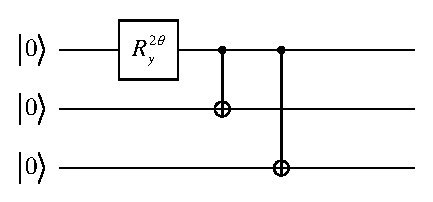
\includegraphics[width=0.5\columnwidth]{net.eps}
\caption{\footnotesize{Quantum network for creating a generalized
GHZ state. The input state is $\left\vert 000 \right\rangle$.
$R_y^{2\theta}$ denotes a rotation of an angle $2\theta$ along Y
axis, following by two controlled-not (CNOT) gates. The output state
is a generalized GHZ state $\cos\theta\left\vert 000
\right\rangle+\sin\theta\left\vert 111 \right\rangle$.}}
\end{figure}

\begin{figure}[h] \centering
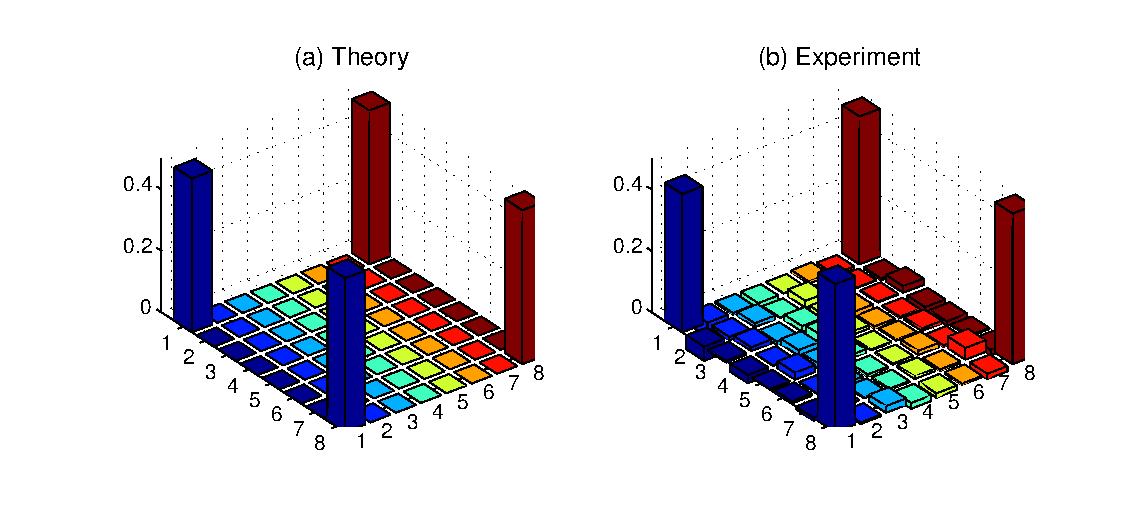
\includegraphics[width=0.8\columnwidth]{tomo.eps}
\caption{\footnotesize{Theoretical (a) and experimental (b) density
matrices of the standard GHZ state $(\left\vert 000
\right\rangle+\left\vert 111 \right\rangle)/{\sqrt{2}}$. }}
\end{figure}

\begin{figure}[h] \centering
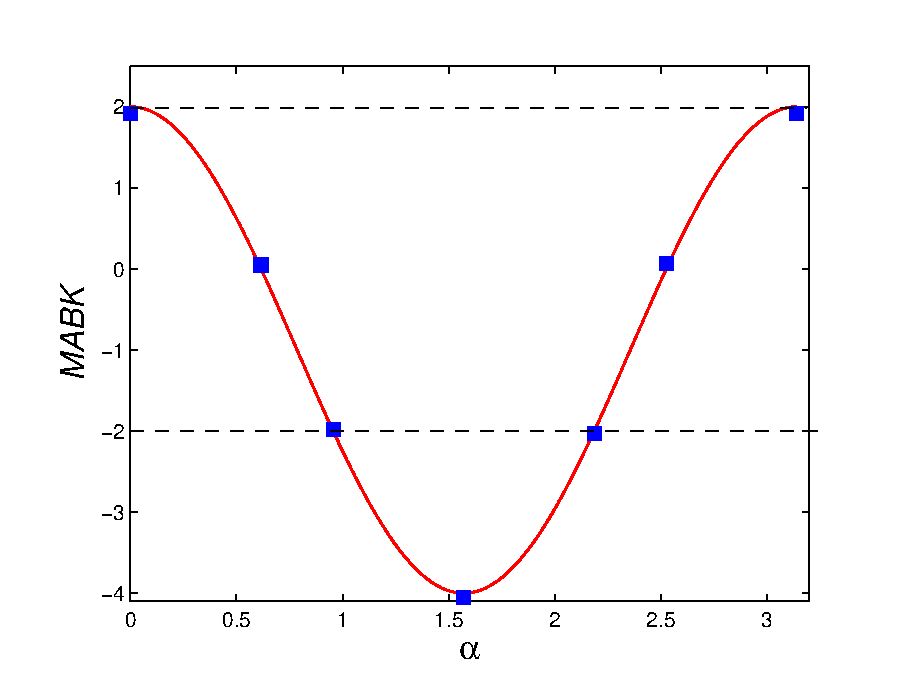
\includegraphics[width=0.5\columnwidth]{MABK.eps}
\caption{\footnotesize{Experimental test of the MABK inequality for
a standard GHZ state. The red thick line stands for the theoretical
expectation, and the blue square stands for the experimental data.}}
\end{figure}

\begin{figure}[h]
\begin{center}
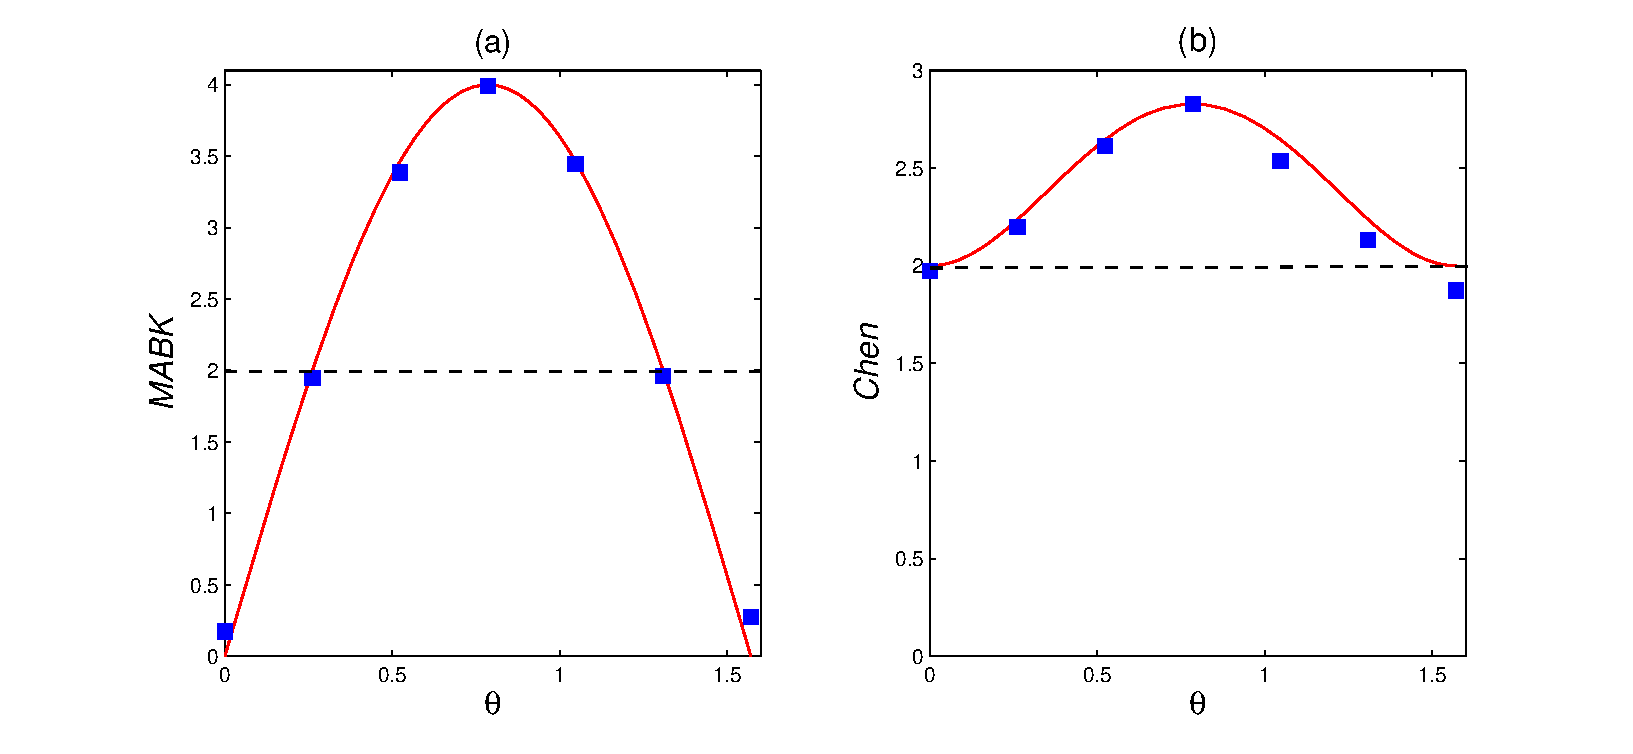
\includegraphics[width=0.8\textwidth]{MABK-Chen.eps}
\caption{\footnotesize{For the generalized GHZ states, (a) the
values of $\mathcal{B}_{MABK}$ as a function of $\theta$, (b) the
values of $\mathcal{B}_{Chen}$ as a function of $\theta$. The red
thick line stands for the theoretical expectation, and the blue
square stands for the experiment data.}}
\end{center}
\end{figure}
\end{document}
